%!TeX encoding = UTF-8
%!TeX program = xelatex
\documentclass[notheorems, aspectratio=1610]{beamer}
% aspectratio: 1610, 149, 54, 43(default), 32
\usepackage[UTF8,noindent]{ctexcap}%引入中文
\usepackage{pythonhighlight}
%\usepackage{ctex}
\usepackage{latexsym}
\usepackage{amsmath,amssymb}
\usepackage{mathtools}
\usepackage{color,xcolor}
\usepackage{graphicx}
\usepackage{algorithm}
\usepackage{amsthm}
\usepackage{lmodern} % 解决 font warning
% \usepackage[UTF8]{ctex}
\usepackage{animate} % insert gif

\usepackage{lipsum} % To generate test text 
\usepackage{ulem} % 下划线,波浪线
\usepackage{geometry}
\usepackage{listings} % display code on slides; don't forget [fragile] option after \begin{frame}
\usepackage{caption}
% ----------------------------------------------
% tikx
\usepackage{framed}
\usepackage{tikz}
\usepackage{pgf}
\usetikzlibrary{calc,trees,positioning,arrows,chains,shapes.geometric,%
    decorations.pathreplacing,decorations.pathmorphing,shapes,%
    matrix,shapes.symbols}
\pgfmathsetseed{1} % To have predictable results
% Define a background layer, in which the parchment shape is drawn
\pgfdeclarelayer{background}
\pgfsetlayers{background,main}

\definecolor{seagull}{HTML}{CDCDCD}
% define styles for the normal border and the torn border
\tikzset{
  normal border/.style={seagull, decorate, 
     decoration={random steps, segment length=2.5cm, amplitude=.7mm}},
  torn border/.style={seagull, decorate, 
     decoration={random steps, segment length=.5cm, amplitude=1.7mm}}}

% Macro to draw the shape behind the text, when it fits completly in the
% page
\def\parchmentframe#1{
\tikz{
  \node[inner sep=1em] (A) {#1};  % Draw the text of the node
  \begin{pgfonlayer}{background}  % Draw the shape behind
  \fill[normal border] 
        (A.south east) -- (A.south west) -- 
        (A.north west) -- (A.north east) -- cycle;
  \end{pgfonlayer}}}

% Macro to draw the shape, when the text will continue in next page
\def\parchmentframetop#1{
\tikz{
  \node[inner sep=2em] (A) {#1};    % Draw the text of the node
  \begin{pgfonlayer}{background}    
  \fill[normal border]              % Draw the ``complete shape'' behind
        (A.south east) -- (A.south west) -- 
        (A.north west) -- (A.north east) -- cycle;
  \fill[torn border]                % Add the torn lower border
        ($(A.south east)-(0,.2)$) -- ($(A.south west)-(0,.2)$) -- 
        ($(A.south west)+(0,.2)$) -- ($(A.south east)+(0,.2)$) -- cycle;
  \end{pgfonlayer}}}

% Macro to draw the shape, when the text continues from previous page
\def\parchmentframebottom#1{
\tikz{
  \node[inner sep=2em] (A) {#1};   % Draw the text of the node
  \begin{pgfonlayer}{background}   
  \fill[normal border]             % Draw the ``complete shape'' behind
        (A.south east) -- (A.south west) -- 
        (A.north west) -- (A.north east) -- cycle;
  \fill[torn border]               % Add the torn upper border
        ($(A.north east)-(0,.2)$) -- ($(A.north west)-(0,.2)$) -- 
        ($(A.north west)+(0,.2)$) -- ($(A.north east)+(0,.2)$) -- cycle;
  \end{pgfonlayer}}}

% Macro to draw the shape, when both the text continues from previous page
% and it will continue in next page
\def\parchmentframemiddle#1{
\tikz{
  \node[inner sep=2em] (A) {#1};   % Draw the text of the node
  \begin{pgfonlayer}{background}   
  \fill[normal border]             % Draw the ``complete shape'' behind
        (A.south east) -- (A.south west) -- 
        (A.north west) -- (A.north east) -- cycle;
  \fill[torn border]               % Add the torn lower border
        ($(A.south east)-(0,.2)$) -- ($(A.south west)-(0,.2)$) -- 
        ($(A.south west)+(0,.2)$) -- ($(A.south east)+(0,.2)$) -- cycle;
  \fill[torn border]               % Add the torn upper border
        ($(A.north east)-(0,.2)$) -- ($(A.north west)-(0,.2)$) -- 
        ($(A.north west)+(0,.2)$) -- ($(A.north east)+(0,.2)$) -- cycle;
  \end{pgfonlayer}}}

% Define the environment which puts the frame
% In this case, the environment also accepts an argument with an optional
% title (which defaults to ``Example'', which is typeset in a box overlaid
% on the top border
\newenvironment{parchment}[1][Example]{%
  \def\FrameCommand{\parchmentframe}%
  \def\FirstFrameCommand{\parchmentframetop}%
  \def\LastFrameCommand{\parchmentframebottom}%
  \def\MidFrameCommand{\parchmentframemiddle}%
  \vskip\baselineskip
  \MakeFramed {\FrameRestore}
  \noindent\tikz\node[inner sep=1ex, draw=black, fill=seagull,
          anchor=west, overlay] at (0em, 1em) {\sffamily#1};\par}%
{\endMakeFramed}

% ----------------------------------------------

\mode<presentation>{
    \usetheme[right]{Berkeley}
    % Boadilla CambridgeUS
    % default Antibes Berlin Copenhagen
    % Madrid Montpelier Ilmenau Malmoe
    % Berkeley Singapore Warsaw
    \usecolortheme{seagull}
    % beetle, beaver, orchid, whale, dolphin
    \useoutertheme{infolines}
    % infolines miniframes shadow sidebar smoothbars smoothtree split tree
    \useinnertheme{circles}
    % circles, rectanges, rounded, inmargin
}
% 设置 block 颜色
\setbeamercolor{block title}{bg=seagull,fg=white}
\setbeamercolor*{block title}{parent=structure,bg=black!70!gray,fg=seagull}

\newcommand{\reditem}[1]{\setbeamercolor{item}{fg=red}\item #1}

% 缩放公式大小
\newcommand*{\Scale}[2][4]{\scalebox{#1}{\ensuremath{#2}}}

% 解决 font warning
\renewcommand\textbullet{\ensuremath{\bullet}}

% ---------------------------------------------------------------------
% flow chart
\tikzset{
    >=stealth',
    punktchain/.style={
        rectangle, 
        rounded corners, 
        % fill=black!10,
        draw=white, very thick,
        text width=6em,
        minimum height=2em, 
        text centered, 
        on chain
    },
    largepunktchain/.style={
        rectangle,
        rounded corners,
        draw=white, very thick,
        text width=10em,
        minimum height=2em,
        on chain
    },
    line/.style={draw, thick, <-},
    element/.style={
        tape,
        top color=white,
        bottom color=blue!50!black!60!,
        minimum width=6em,
        draw=blue!40!black!90, very thick,
        text width=6em, 
        minimum height=2em, 
        text centered, 
        on chain
    },
    every join/.style={->, thick,shorten >=1pt},
    decoration={brace},
    tuborg/.style={decorate},
    tubnode/.style={midway, right=2pt},
    font={\fontsize{10pt}{12}\selectfont},
}
% ---------------------------------------------------------------------

% code setting
% \lstset{
%     language=Python,
%     basicstyle=\ttfamily\footnotesize,
%     keywordstyle=\color{red},
%     breaklines=true,
%     xleftmargin=2em,
%     numbers=left,
%     numberstyle=\color[RGB]{222,155,81},
%     frame=leftline,
%     tabsize=4,
%     breakatwhitespace=false,
%     showspaces=false,               
%     showstringspaces=false,
%     showtabs=false,
%     morekeywords={Str, Num, List},
% }
% 用来设置附录中代码的样式

% \lstset{
%     basicstyle          =   \sffamily,          % 基本代码风格
%     keywordstyle        =   \bfseries,          % 关键字风格
%     commentstyle        =   \rmfamily\itshape,  % 注释的风格,斜体
%     stringstyle         =   \ttfamily,  % 字符串风格
%     flexiblecolumns,                % 别问为什么,加上这个
%     numbers             =   left,   % 行号的位置在左边
%     showspaces          =   false,  % 是否显示空格,显示了有点乱,所以不现实了
%     numberstyle         =   \zihao{-5}\ttfamily,    % 行号的样式,小五号,tt等宽字体
%     showstringspaces    =   false,
%     captionpos          =   t,      % 这段代码的名字所呈现的位置,t指的是top上面
%     frame               =   lrtb,   % 显示边框
%     numberstyle= \tiny, 
% }

% \lstdefinestyle{Python}{
%     language        =   Python, % 语言选Python
%     basicstyle      =   \zihao{-5}\ttfamily,
%     numberstyle     =   \zihao{-5}\ttfamily,
%     keywordstyle    =   \color{blue},
%     keywordstyle    =   [2] \color{teal},
%     stringstyle     =   \color{magenta},
%     commentstyle    =   \color{red}\ttfamily,
%     breaklines      =   true,   % 自动换行,建议不要写太长的行
%     columns         =   fixed,  % 如果不加这一句,字间距就不固定,很丑,必须加
%     basewidth       =   0.5em,
% }

% ---------------------------------------------------------------------

%% preamble
\title[持续化部署的高速公路车流量预测系统]{持续化部署的高速公路车流量预测系统}
%\subtitle{持续化部署的高速公路车流量预测系统}
\author{李子铭}
\institute[NJU]{liziming-cn@qq.com}
%\setbeamersize{sidebar width right=0pt}
%\linespread{1.5} % 行间距设置1.5

% -------------------------------------------------------------

\begin{document}

%% title frame
\begin{frame}[plain]
    \addtolength\textwidth{1.5cm} 
    \setlength\hsize{\textwidth} 
    \setlength\columnwidth{\textwidth}
    \titlepage
    %\maketitle
   
\end{frame}
\begin{frame}           %生成目录页,目录太长时加选项[shrink]
        \addtocounter{framenumber}{-2}%---------位置放在beginframe之后,不然无效
        \frametitle{目录}
        \thispagestyle{empty}
        \tableofcontents        % 也可以插入选项 [pausesections]
        %----------------------列目录时,隐藏所有的小节
        %\tableofcontents[hideallsubsections]
\end{frame}
%% normal frame
\section{背景介绍}
\subsection{应用场景}
\begin{frame}
    %\frametitle{应用场景}
    目标:根据已有的公路收费信息,构建一个车流量预测系统:
    \begin{figure}[h] %figure环境,h默认参数是可以浮动,不是固定在当前位置。如果要不浮动,你就可以使用大写float宏包的H参数,固定图片在当前位置,禁止浮动。
        \flushleft %左对齐
        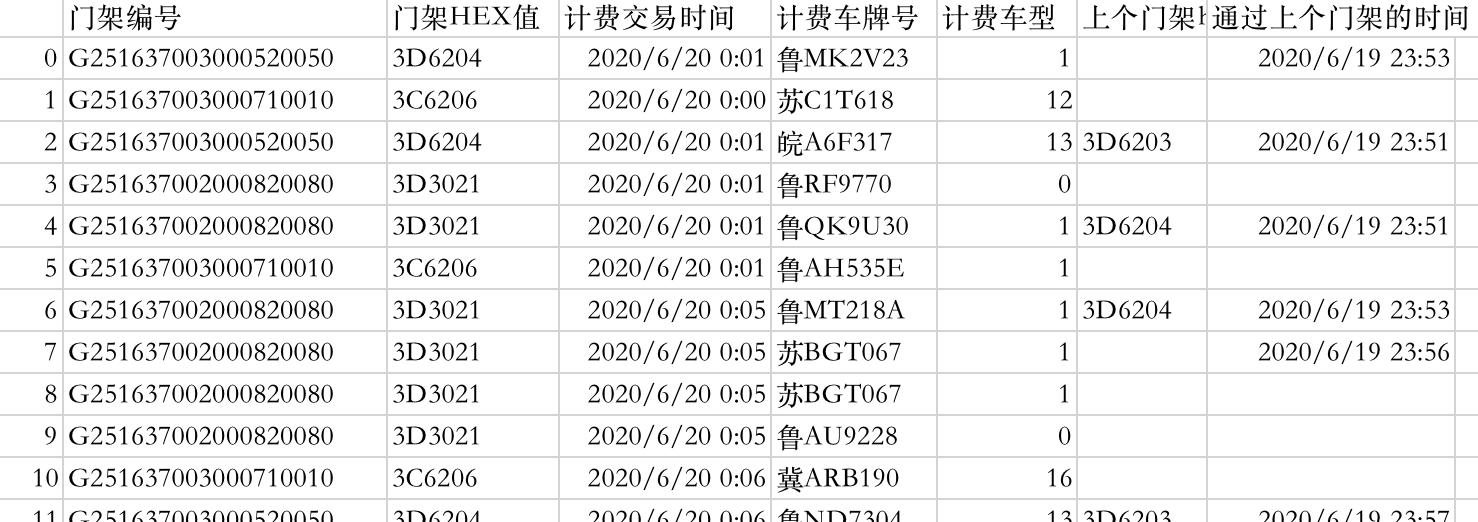
\includegraphics[width=0.8\textwidth]{../材料/pic/计费数据.png} %中括号中的参数是设置图片充满文档的大小,你也可以使用小数来缩小图片的尺寸。
        %\caption{推荐系统} %caption是用来给图片加上图题的
        %\label{wolf} %这是添加标签,方便在文章中引用图片。
    \end{figure}%figure环境
    \begin{block}{思考:怎样通过计费收费信息,去构建一个车流量预测系统?}
        机器学习应用:以机器学习算法为基础,完成从数据分析开始、到最后的模型服务发布等流程
    \end{block}
\end{frame}

\subsection{机器学习应用的生命周期}
\begin{frame}
    %\frametitle{应用场景}
    一般而言,机器学习应用的生命周期主要分为以下几个步骤:
    \begin{enumerate}
        \item 数据预处理:从原始数据中提取数据集
        \item 模型的训练:利用数据集去进行模型的训练、验证,得到一个效果较优的模型
        \item 模型的发布:将上一步得到的模型部署在后端服务里,提供在线预测的api
    \end{enumerate}
    \begin{block}{思考:怎样把这个流程给流水线化、可持续化?}
        由于整个过程比较繁琐、碎片化,开始研究怎样将模型的训练、部署过程流程化、可持续化,从而解放人力
    \end{block}
\end{frame}
\subsection{机器学习应用可持续部署案例介绍}
\begin{frame}
%分列
\begin{columns}
    %\frametitle{应用场景}
    
    \column{0.4\textwidth}
    \begin{figure}[h] %figure环境,h默认参数是可以浮动,不是固定在当前位置。如果要不浮动,你就可以使用大写float宏包的H参数,固定图片在当前位置,禁止浮动。
        \flushleft %左对齐
        
\includegraphics[width=0.8\textwidth]{../材料/pic/googlepaly.jpg} %中括号中的参数是设置图片充满文档的大小,你也可以使用小数来缩小图片的尺寸。
        %\caption{推荐系统} %caption是用来给图片加上图题的
        %\label{wolf} %这是添加标签,方便在文章中引用图片。
    \end{figure}%figure环境
    \column{0.6\textwidth}
    比如Google Play的在线推荐系统:
    \begin{itemize}

        \item 升级成一个持续化模型训练、模型更新的pipline
        \item 每天会收集当天的用户点击数据进行模型的更新
        \item 对比原先的推荐系统,加快了迭代速度、减少了技术复杂性、提高了模型质量
        \item 下载率上升2\%
    \end{itemize}
\end{columns}

\end{frame}


\section{相关技术}
\subsection{TFX:端到端的用于部署生产型机器学习的流水线}
\begin{frame}
    \large TFX(Tensorflow Extended):端到端的用于部署生产型机器学习的流水线:
    \begin{itemize}
        \item 将之前说的模型整个工作流程组件化,提供工具包,搭建pipline
        \item pipline的执行由相应的编排器执行,例如Apache Airflow,Apache Beam和Kubeflow Pipelines
        \item pipline间的数据传递、存储交由相应的数据库服务管理
    \end{itemize} 
    \par 目的:针对机器学习模型的训练到部署、再到演化更新这一场景,提供一套标准的组件,简化系统的配置,从而大幅度降低系统搭建时间。
\end{frame}

\begin{frame}
    \large 目前,TFX提供的标准组件主要有以下几个:
    \begin{figure}[h] %figure环境,h默认参数是可以浮动,不是固定在当前位置。如果要不浮动,你就可以使用大写float宏包的H参数,固定图片在当前位置,禁止浮动。
        \centering
        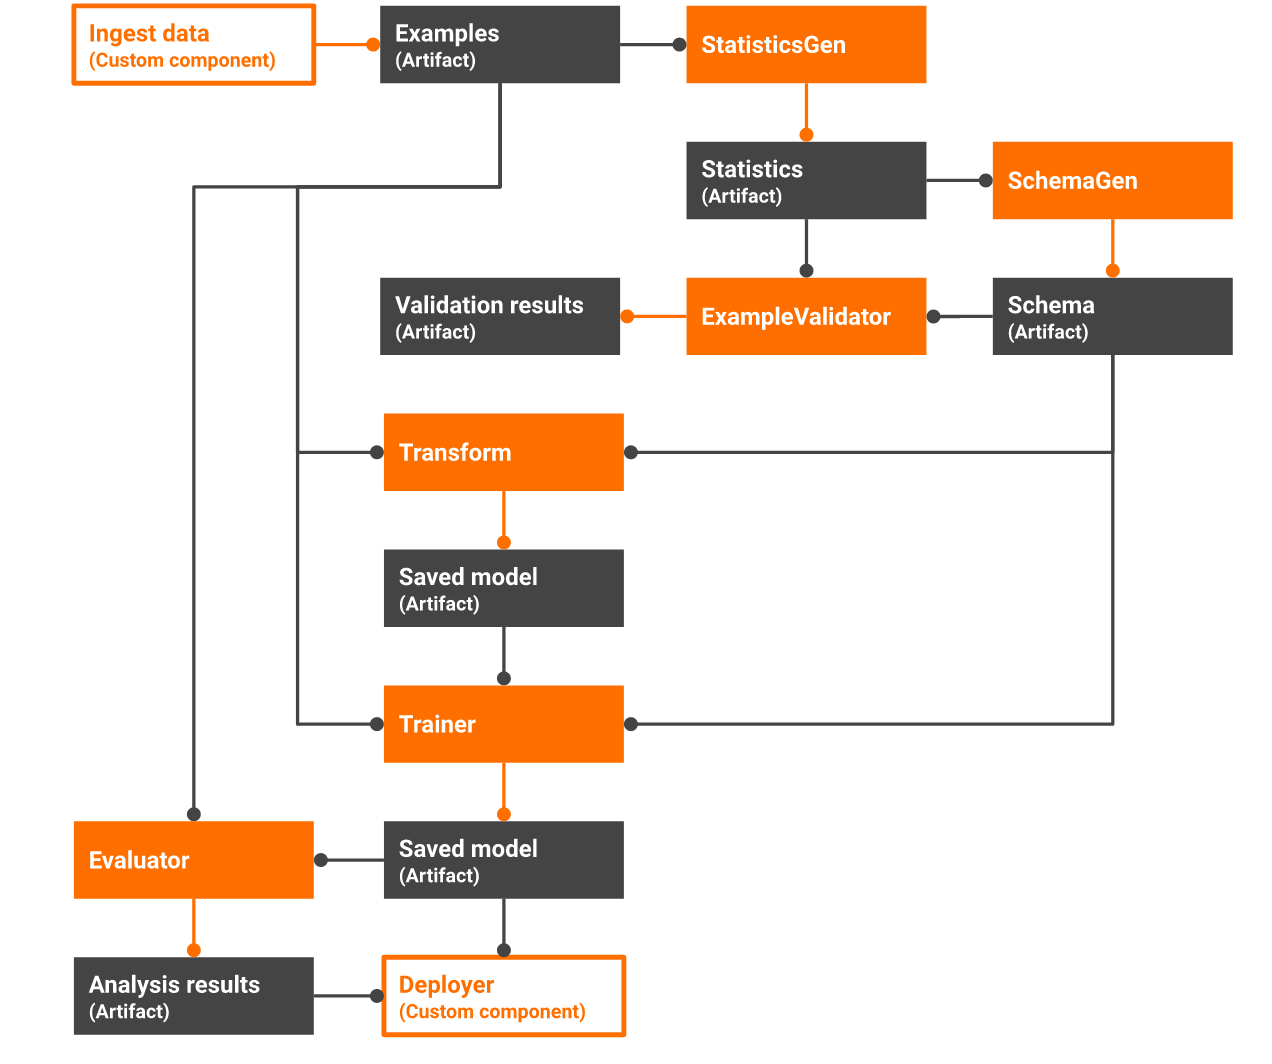
\includegraphics[width=0.7\textwidth]{../材料/pic/components.png} %中括号中的参数是设置图片充满文档的大小,你也可以使用小数来缩小图片的尺寸。
        %\caption{推荐系统} %caption是用来给图片加上图题的
        %\label{wolf} %这是添加标签,方便在文章中引用图片。
    \end{figure}%figure环境

\end{frame}

\begin{frame}
    \large TFX pipline 组件的组成结构
    \begin{itemize}
        \item specification :指明组件的输入输出,两种输入:Artifact、Parameter,一种输出OutputDict
        \item executor:拿到输入参数后,该怎么执行?(一个处理函数,接收Artifact、Parameter)
        \item interface:将specification与executor进行封装成组件
    \end{itemize}
    \begin{figure}[h] %figure环境,h默认参数是可以浮动,不是固定在当前位置。如果要不浮动,你就可以使用大写float宏包的H参数,固定图片在当前位置,禁止浮动。
    \centering %居中对齐
    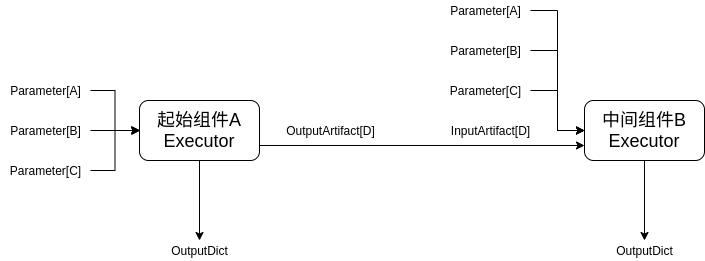
\includegraphics[width=1\textwidth]{../材料/pic/组件数据流.png} %中括号中的参数是设置图片充满文档的大小,你也可以使用小数来缩小图片的尺寸。
    %\caption{推荐系统} %caption是用来给图片加上图题的
    %\label{wolf} %这是添加标签,方便在文章中引用图片。
    \end{figure}%figure环境
\end{frame}

% \begin{frame}
%     \large 使用组件的两个关键点:
%     \begin{enumerate}
%         \item 数据的存储与传递
        
%         \item 组件的执行流程
%     \end{enumerate}

% \end{frame}
\begin{frame}
    \large 组件的执行流程:
    \begin{enumerate}
        \item driver从metadata store中检索需要的Artifact数据、Parameter参数,将其传递给组件
        \item executor执行组件事先定义好的处理逻辑
        \item publisher将specification与executor执行的结果存储在metadata store里
    \end{enumerate}
    \begin{figure}[h] %figure环境,h默认参数是可以浮动,不是固定在当前位置。如果要不浮动,你就可以使用大写float宏包的H参数,固定图片在当前位置,禁止浮动。
        \centering %居中对齐
        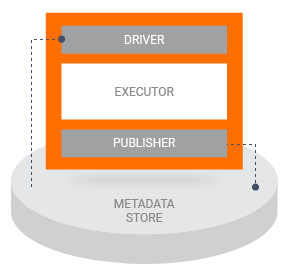
\includegraphics[width=0.4\textwidth]{../材料/pic/component.png} %中括号中的参数是设置图片充满文档的大小,你也可以使用小数来缩小图片的尺寸。
        %\caption{推荐系统} %caption是用来给图片加上图题的
        %\label{wolf} %这是添加标签,方便在文章中引用图片。
    \end{figure}%figure环境
\end{frame}
\begin{frame}[fragile]
    
    \large 举个例子:
    % \begin{lstlisting}[language=Python]
    %     @component  #组件的接口:将组件规范与组件的执行器进行封装
    %     def MyExampleGen(
    %         examples: OutputArtifact[Examples], #组件规范:指定组件的输入输出数据类型,以及其他参数
    %         es_index: Parameter[str],
    %         param: Parameter[str],
    %         host:Parameter[str],
    %         port:Parameter[int],
    % \end{lstlisting}
    \begin{python}[]
@component  #组件的接口:将组件规范与组件的执行器进行封装
def MyExampleGen(
    examples: OutputArtifact[Examples], #组件规范:指定组件的输入输出数据类型,以及其他参数
    es_index: Parameter[str],param: Parameter[str],
    host:Parameter[str],port:Parameter[int],
    gte: Parameter[str],lte: Parameter[str],
    debug:Parameter[str]='False'
    )->OutputDict(test=str):
    if(debug=='True'):
        return {
        }
    param=json.loads(param)       #组件的执行器:拿到输入参数后,该怎么执行?
    data=getVolumeFromES(host,es_index,port,gte,lte)
    table=pd.DataFrame(data,columns=['计费交易时间','门架HEX值','门架编号','doc_count'])
    ……
    return {
        'test'=123
    }
    \end{python}
\end{frame}
\subsection{其他的pipline}
\begin{frame}
    另一种pipline,数据与模型流程分离:
    \begin{figure}[h] %figure环境,h默认参数是可以浮动,不是固定在当前位置。如果要不浮动,你就可以使用大写float宏包的H参数,固定图片在当前位置,禁止浮动。
        \centering %居中对齐
        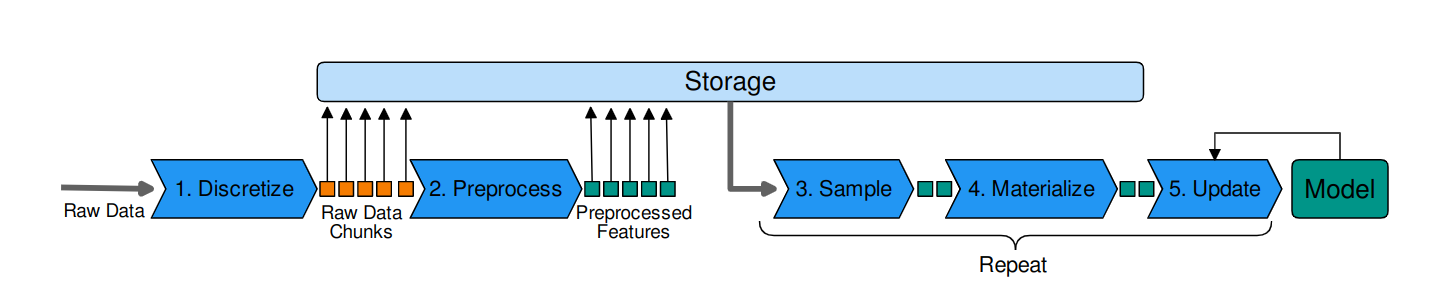
\includegraphics[width=1\textwidth]{../材料/pic/a_pipline.png} %中括号中的参数是设置图片充满文档的大小,你也可以使用小数来缩小图片的尺寸。
        %\caption{推荐系统} %caption是用来给图片加上图题的
        %\label{wolf} %这是添加标签,方便在文章中引用图片。
    \end{figure}%figure环境
    \begin{itemize}
        \item 数据预处理:将raw data转化为feature data,并储存
        \item 模型训练与发布:从存储系统里取出feature data,进行模型训练、发布
    \end{itemize}
\end{frame}
\section{系统结构}
\subsection{系统结构图}
\begin{frame}
    \begin{columns}
        \column{0.5\textwidth}
        \large 系统的整体架构图
        \begin{figure}[h] %figure环境,h默认参数是可以浮动,不是固定在当前位置。如果要不浮动,你就可以使用大写float宏包的H参数,固定图片在当前位置,禁止浮动。
            \flushleft %左对齐
            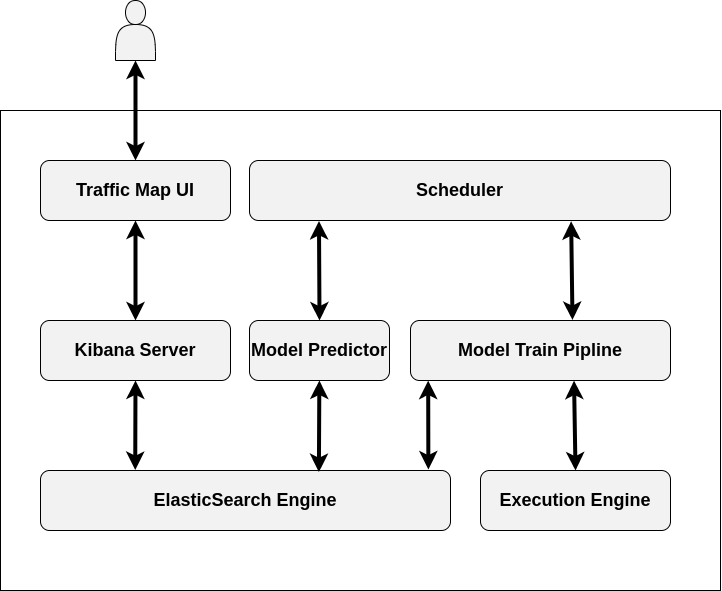
\includegraphics[width=1\textwidth]{../材料/pic/架构图3.png} %中括号中的参数是设置图片充满文档的大小,你也可以使用小数来缩小图片的尺寸。
            %\caption{推荐系统} %caption是用来给图片加上图题的
            %\label{wolf} %这是添加标签,方便在文章中引用图片。
        \end{figure}%figure环境
        \column{0.5\textwidth}
        \begin{itemize}
            \item scheduler:负责执行机器学习应用的pipline;同时负责调用predictor
            \item model predictor:负责预测车流量,并将结果写入数据库
            \item train pipline:负责执行一次数据处理、模型训练流程,生成新的模型
            \item Map UI、Kibana:提供车流量数据的可视化界面
            \item ElasticSearch:提供数据库服务
        \end{itemize}
        
    \end{columns}
    
\end{frame}
\subsection{交互部分}
\begin{frame}
    \large 车流量数据可视化
    \begin{figure}[h] %figure环境,h默认参数是可以浮动,不是固定在当前位置。如果要不浮动,你就可以使用大写float宏包的H参数,固定图片在当前位置,禁止浮动。
        \centering %居中对齐
        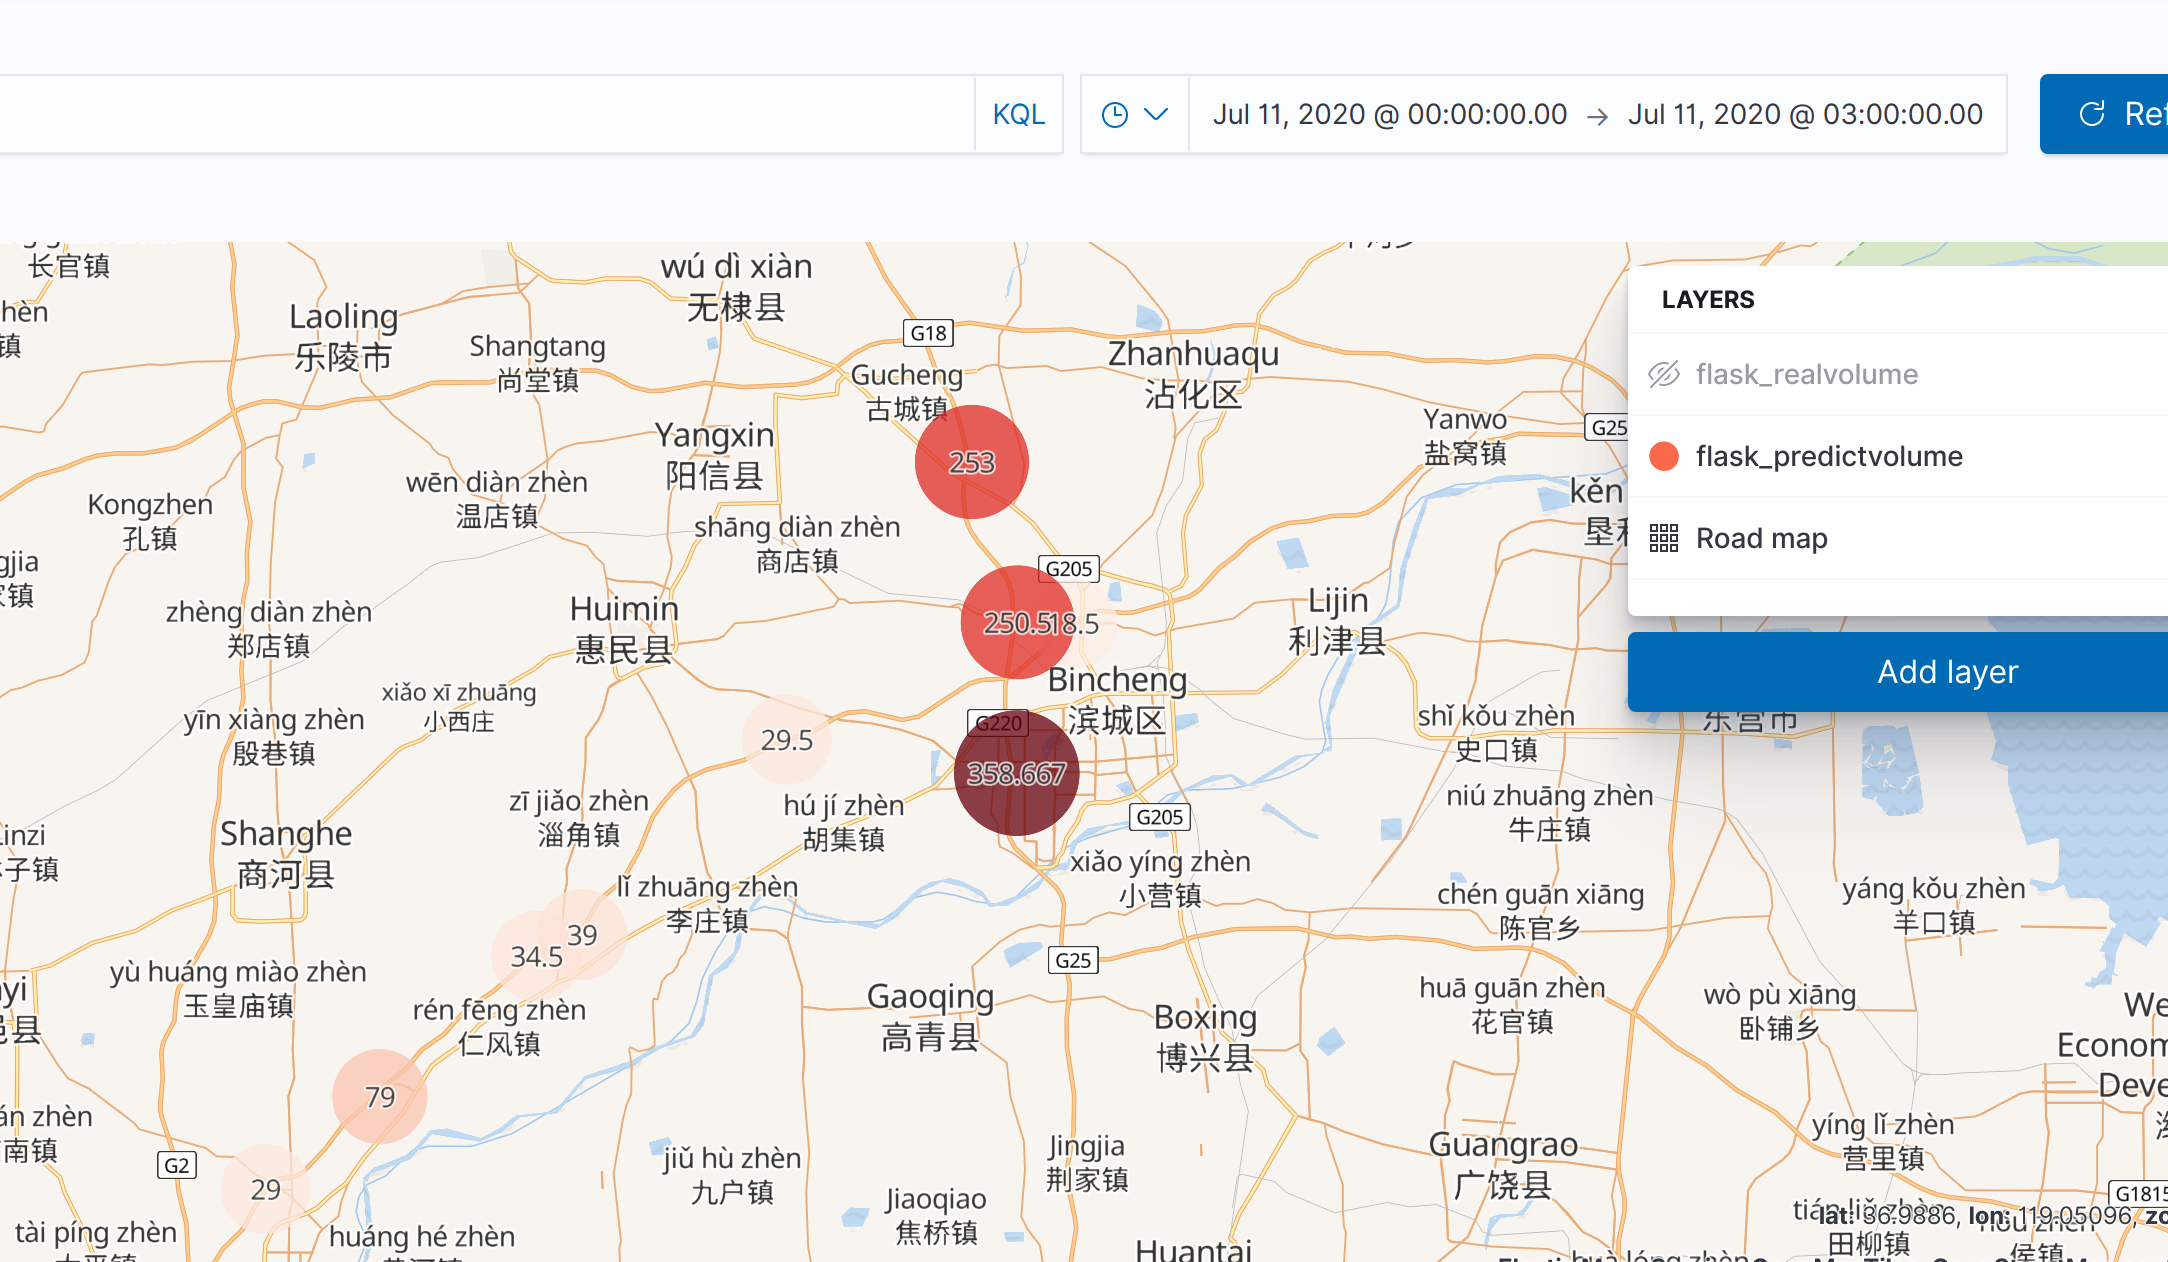
\includegraphics[width=1\textwidth]{../材料/pic/kinbana.png} %中括号中的参数是设置图片充满文档的大小,你也可以使用小数来缩小图片的尺寸。
        %\caption{推荐系统} %caption是用来给图片加上图题的
        %\label{wolf} %这是添加标签,方便在文章中引用图片。
    \end{figure}%figure环境
\end{frame}
\begin{frame}
    scheduler:负责调用Predictor与train pipline
    \begin{itemize}
        \item 调用Predictor\par
        \small 什么时候进行预测?每天?每小时?
        \begin{enumerate}
            \item 从使用的model考虑:假定要预测每小时的车流量,model根据前72小时预测后24小时的预测,那么每次只能使用过去72小时的数据来进行预测,否则就要使用预测出来的数据作为历史数据,这是不合理的
            \item 从用户的角度考虑:用户来到web页面,看到的永远是那一时刻的数据,无需过多的进行预测
        \end{enumerate}
        
        
        
    \end{itemize}
    
\end{frame}
\subsection{scheduler}
\begin{frame}
    scheduler:负责调用Predictor与train pipline
    \begin{itemize}
        \item 调用train pipline\par
        \small 什么时候进行模型的更新演替?每次更新演替是否有必要?
        \begin{enumerate}
            \item 从计算复杂性考虑:从数据处理,到模型训练、验证,这是一个耗时较漫长的过程,也许是几个小时,也许是几天
            \item 从车流量数据的周期性来看:车流量变化在短时期内不会有过大的波动,具有一定的周期性、
            \item 从每个阶段性部署的模型来看:模型总是在一定时期内是可信的,效果是较优的
        \end{enumerate}
    \end{itemize}
    \begin{figure}[h] %figure环境,h默认参数是可以浮动,不是固定在当前位置。如果要不浮动,你就可以使用大写float宏包的H参数,固定图片在当前位置,禁止浮动。
        \centering %居中对齐
        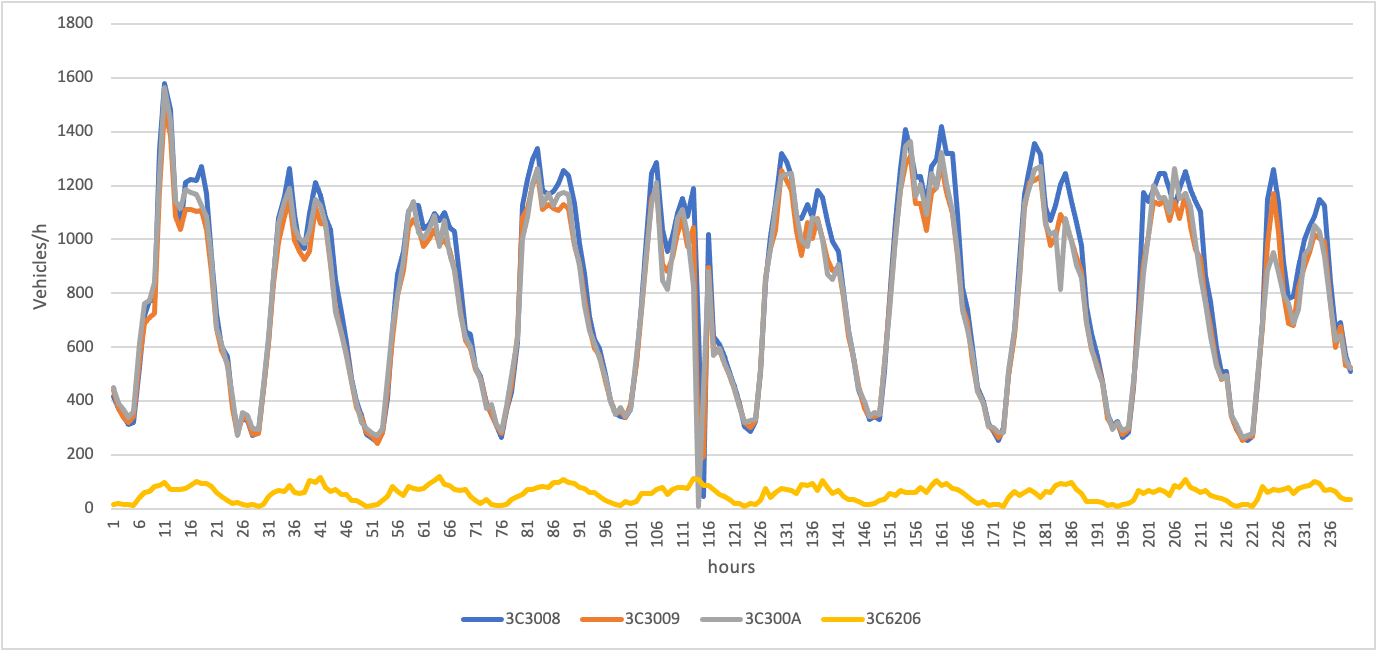
\includegraphics[width=0.8\textwidth]{../材料/pic/10天车流量.png} %中括号中的参数是设置图片充满文档的大小,你也可以使用小数来缩小图片的尺寸。
        %\caption{推荐系统} %caption是用来给图片加上图题的
        %\label{wolf} %这是添加标签,方便在文章中引用图片。
    \end{figure}%figure环境
\end{frame}
\begin{frame}
    scheduler:负责调用Predictor与train pipline
    \begin{itemize}
        \item 调用train pipline的时间策略\par
        \begin{enumerate}
            \item 动态:使用一个数学模型,每次执行pipline,会记录执行起始时间、这个运行花费时间等信息,动态地决定下一次调用的时间点
            \item 静态:设置循环执行的周期值,定时调用
        \end{enumerate}
        \item 调用train pipline的必要性检测\par
        每次到达时间点,不会立刻去执行更新操作,需要根据过去一段时间内的模型表现来进行判断
        \par
        \hspace*{\fill}
        \par
        判断指标:
        \begin{enumerate}
            \item MAPE
            \item MAE
            \item RMSE
        \end{enumerate}
    \end{itemize}
\end{frame}
\subsection{pipline}
\begin{frame}
    \Large pipline组件流程
    \newline
    \begin{figure}[h] %figure环境,h默认参数是可以浮动,不是固定在当前位置。如果要不浮动,你就可以使用大写float宏包的H参数,固定图片在当前位置,禁止浮动。
        \centering %居中对齐
        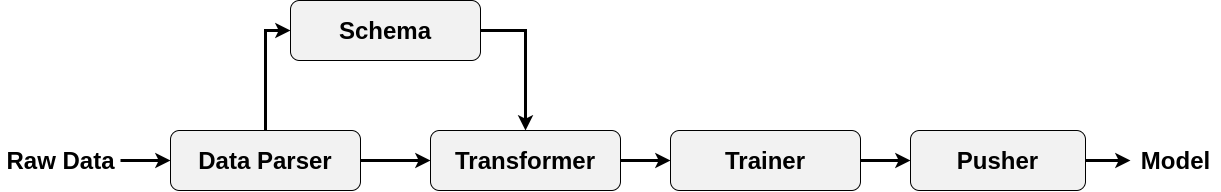
\includegraphics[width=1\textwidth]{../材料/pic/pipline.png} %中括号中的参数是设置图片充满文档的大小,你也可以使用小数来缩小图片的尺寸。
        %\caption{推荐系统} %caption是用来给图片加上图题的
        %\label{wolf} %这是添加标签,方便在文章中引用图片。
    \end{figure}%figure环境
\end{frame}
\begin{frame}
    \Large pipline组件:data parser
    \newline
    \begin{columns}
        \begin{column}{0.5\textwidth}
            \begin{figure}[h] %figure环境,h默认参数是可以浮动,不是固定在当前位置。如果要不浮动,你就可以使用大写float宏包的H参数,固定图片在当前位置,禁止浮动。
                \centering %居中对齐
                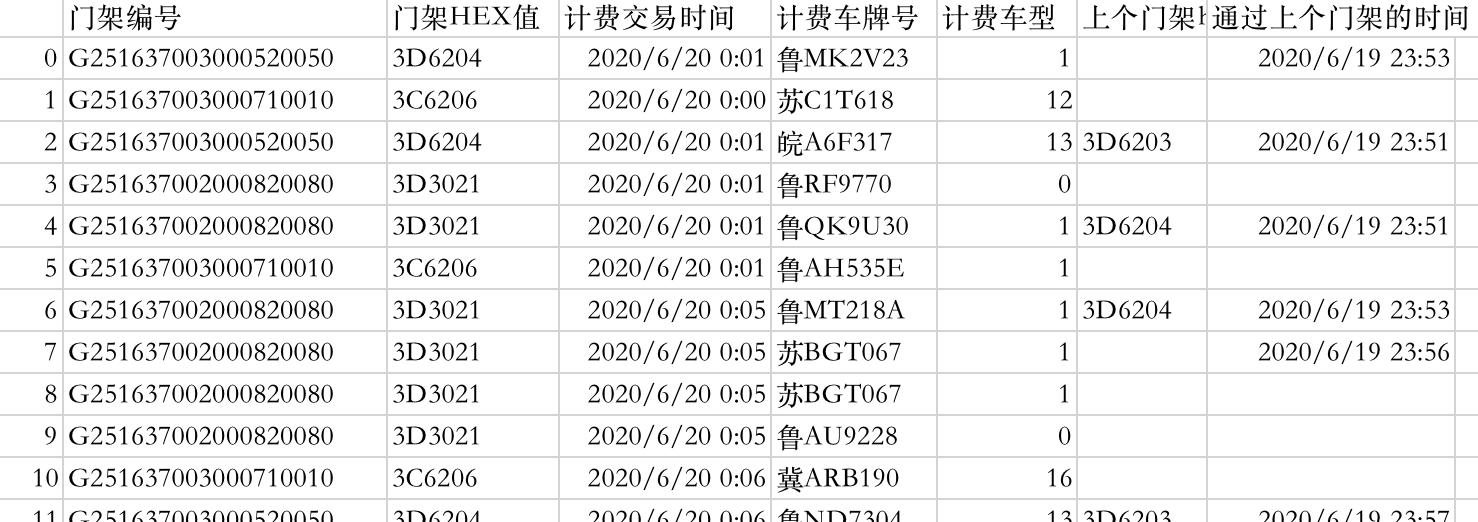
\includegraphics[width=1\textwidth]{../材料/pic/计费数据.png} %中括号中的参数是设置图片充满文档的大小,你也可以使用小数来缩小图片的尺寸。
                %\caption{推荐系统} %caption是用来给图片加上图题的
                %\label{wolf} %这是添加标签,方便在文章中引用图片。
            \end{figure}%figure环境
        \end{column}
        \begin{column}{0.5\textwidth}
            \begin{figure}[h] %figure环境,h默认参数是可以浮动,不是固定在当前位置。如果要不浮动,你就可以使用大写float宏包的H参数,固定图片在当前位置,禁止浮动。
                \centering %居中对齐
                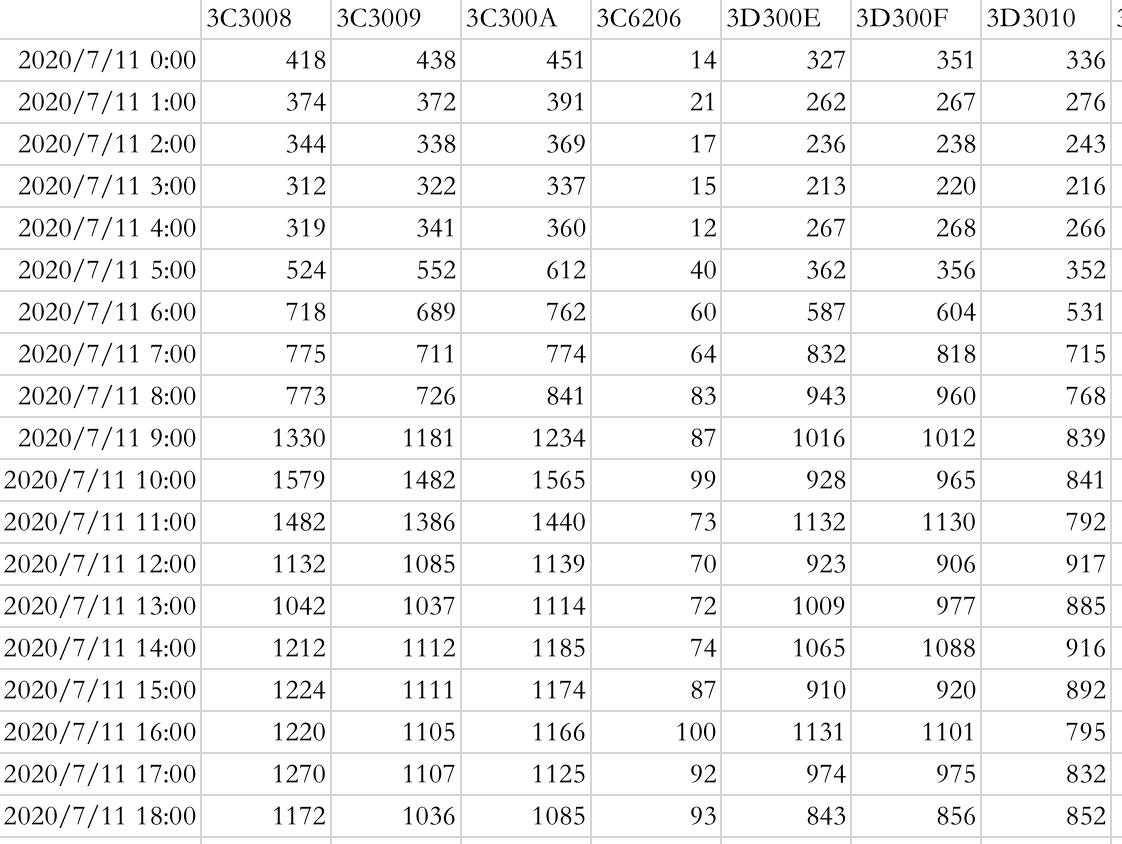
\includegraphics[width=1\textwidth]{../材料/pic/volumes.png} %中括号中的参数是设置图片充满文档的大小,你也可以使用小数来缩小图片的尺寸。
                %\caption{推荐系统} %caption是用来给图片加上图题的
                %\label{wolf} %这是添加标签,方便在文章中引用图片。
            \end{figure}%figure环境
        \end{column}
    \end{columns}
    \normalsize 组件输出:
    \begin{itemize}
        \item 将原始的收费数据转化为每小时的车流量
        \item 同时提供后续模型需要的其他数据
    \end{itemize}
\end{frame}
\begin{frame}
    \Large pipline组件:schema
    \newline
    \normalsize
    \begin{columns}
        
        \begin{column}{0.5\textwidth}
            \begin{figure}[h] %figure环境,h默认参数是可以浮动,不是固定在当前位置。如果要不浮动,你就可以使用大写float宏包的H参数,固定图片在当前位置,禁止浮动。
                \centering %居中对齐
                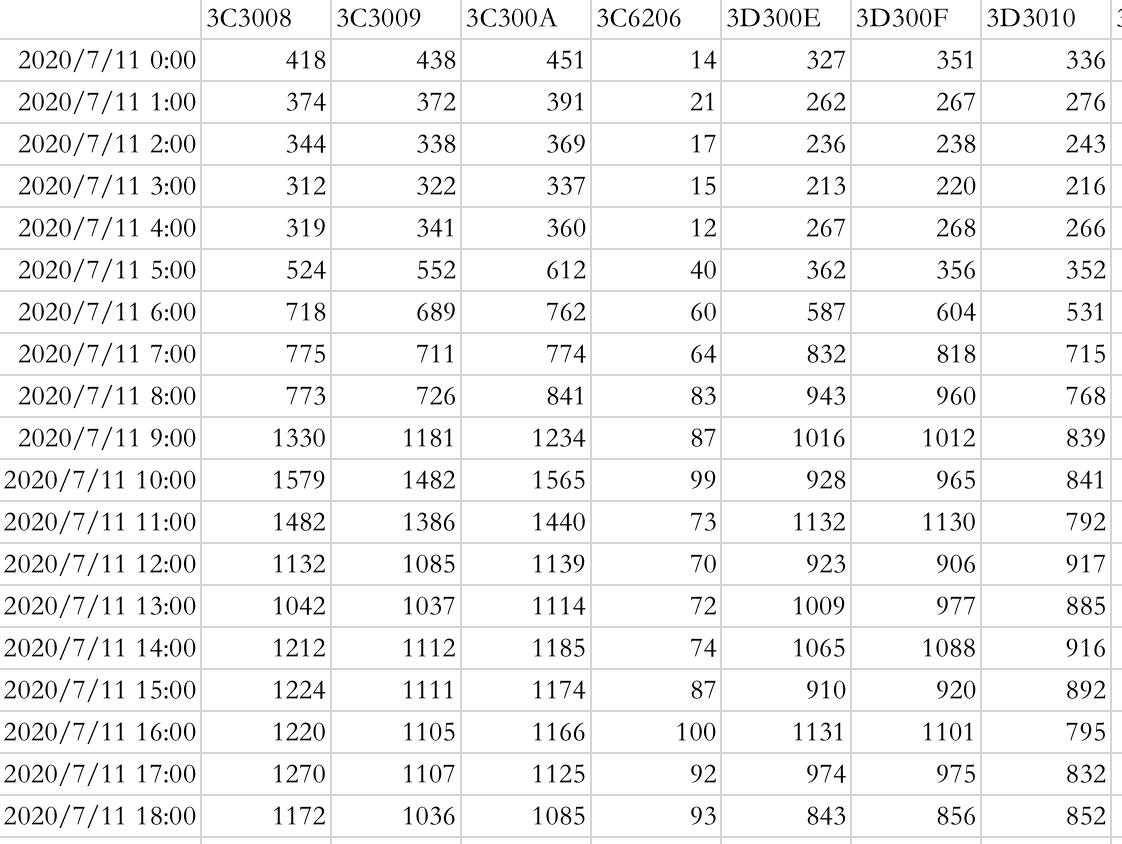
\includegraphics[width=1\textwidth]{../材料/pic/volumes.png} %中括号中的参数是设置图片充满文档的大小,你也可以使用小数来缩小图片的尺寸。
                %\caption{推荐系统} %caption是用来给图片加上图题的
                %\label{wolf} %这是添加标签,方便在文章中引用图片。
            \end{figure}%figure环境
        \end{column}
        \begin{column}{0.5\textwidth}
            每个字段的数据最终应该保存成什么数据类型?
            \begin{itemize}
                \item int
                \item float
                \item double
            \end{itemize}
            \textcolor{black}{考虑到实际应用场景,这里直接将所有字段定义为float}
        \end{column}
    \end{columns}
    组件输出:
    \begin{itemize}
        \item 每个字段应该被转化的数据类型
    \end{itemize}
\end{frame}

\begin{frame}
    \Large pipline组件:transformer
    \newline
    \normalsize
    \begin{columns}
        
        \begin{column}{0.5\textwidth}
            %\animategraphics{2}{./材料/pic/transformer-}{0}{1}
            % \only<1>{ \begin{figure}[h] %figure环境,h默认参数是可以浮动,不是固定在当前位置。如果要不浮动,你就可以使用大写float宏包的H参数,固定图片在当前位置,禁止浮动。
            %     \centering %居中对齐
            %     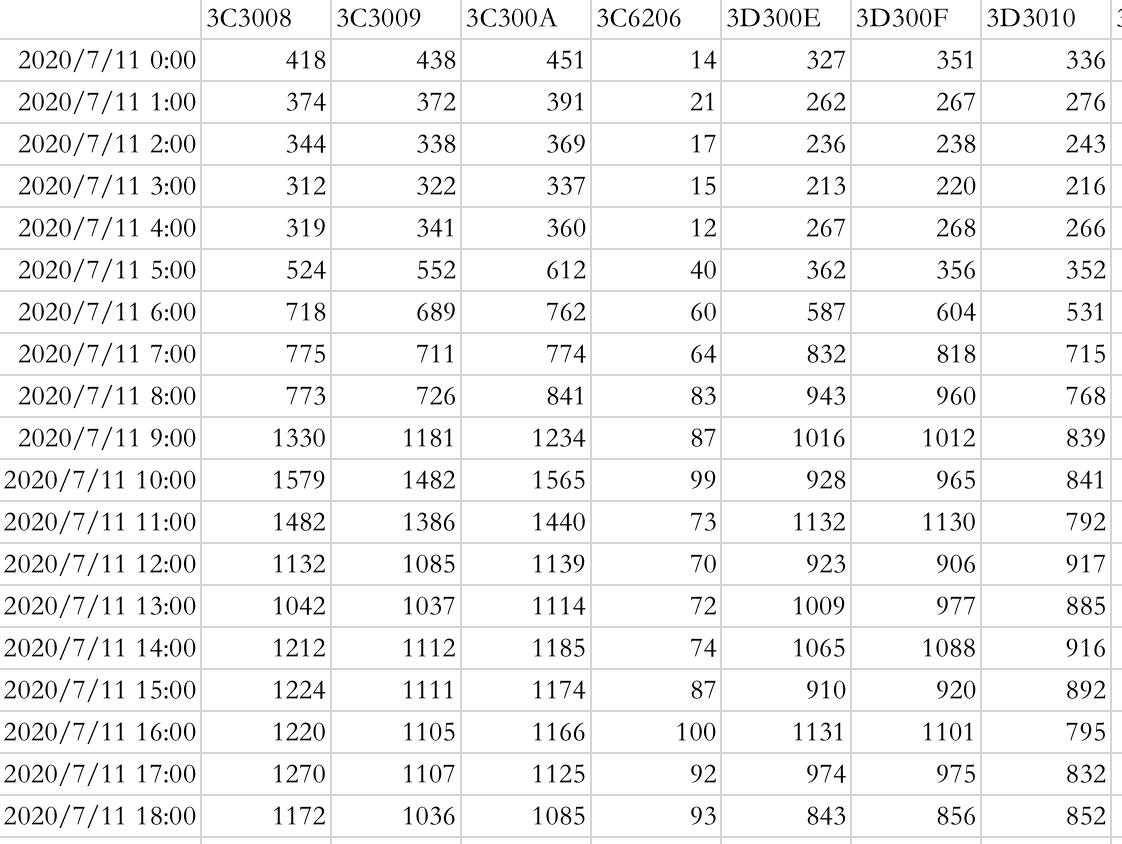
\includegraphics[width=1\textwidth]{../材料/pic/volumes.png} %中括号中的参数是设置图片充满文档的大小,你也可以使用小数来缩小图片的尺寸。
            %     %\caption{推荐系统} %caption是用来给图片加上图题的
            %     %\label{wolf} %这是添加标签,方便在文章中引用图片。
            % \end{figure}%figure环境
            % }
            % \only<2>{\begin{figure}[h] %figure环境,h默认参数是可以浮动,不是固定在当前位置。如果要不浮动,你就可以使用大写float宏包的H参数,固定图片在当前位置,禁止浮动。
            %     \flushleft %左对齐
            %     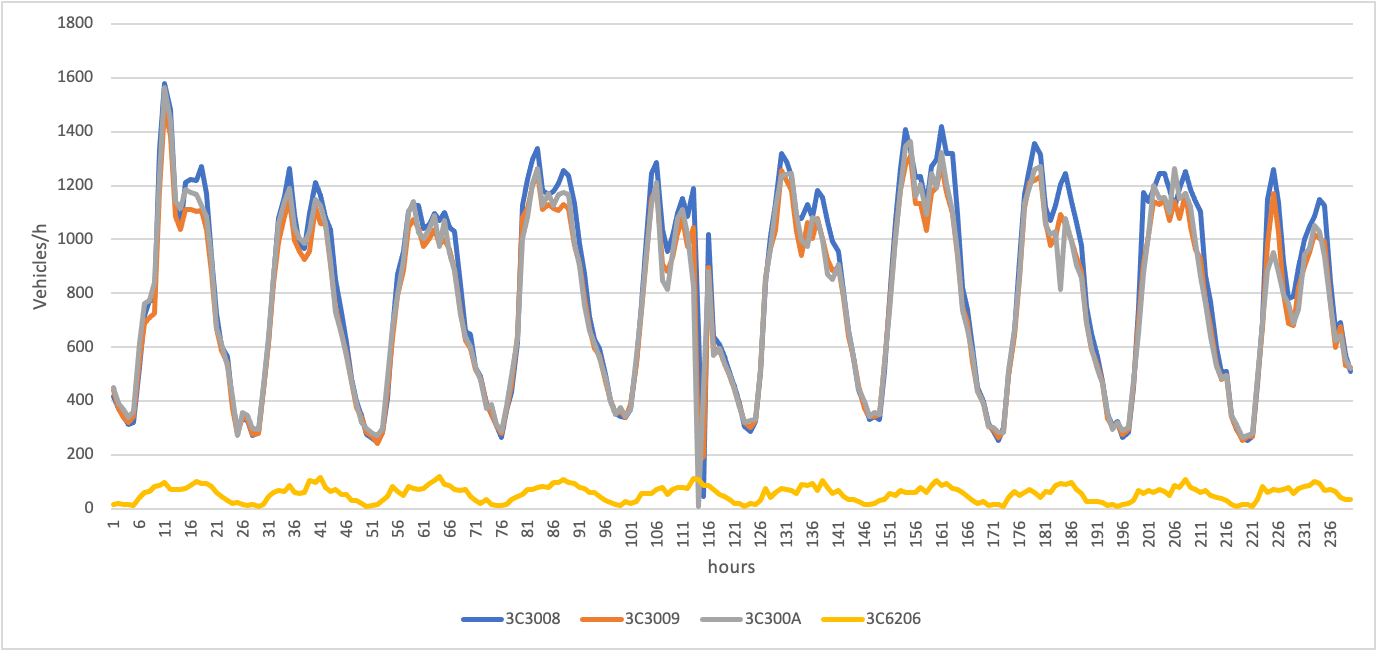
\includegraphics[width=0.8\textwidth]{../材料/pic/10天车流量.png} %中括号中的参数是设置图片充满文档的大小,你也可以使用小数来缩小图片的尺寸。
            %     %\caption{推荐系统} %caption是用来给图片加上图题的
            %     %\label{wolf} %这是添加标签,方便在文章中引用图片。
            % \end{figure}%figure环境
            % }
            \begin{figure}[H] %figure环境,h默认参数是可以浮动,不是固定在当前位置。如果要不浮动,你就可以使用大写float宏包的H参数,固定图片在当前位置,禁止浮动。
                    \centering %居中对齐
                    \includegraphics<1>[width=1\textwidth]{../材料/pic/volumes.png}% 
                    \includegraphics<2>[width=1\textwidth]{../材料/pic/10天车流量.png}%
                    %\caption{推荐系统} %caption是用来给图片加上图题的
                    %\label{wolf} %这是添加标签,方便在文章中引用图片。
            \end{figure}%figure环境
        \end{column}
        \begin{column}{0.5\textwidth}
            在拿到整个路网的各个节点车流量数据后,我们应该怎样利用它?
            \par
            \hspace*{\fill}
            \par
            按照trainer中使用的模型来进行处理:
            \begin{enumerate}
                \item 按照schema中的数据类型——float,将车流量数据进行转换
                \item 根据时间索引,来考虑周期性特征:天、星期、月……
                \item 将构建的特征矩阵进行存储
            \end{enumerate}
        \end{column}
    \end{columns}
    组件输出:
    \begin{itemize}
        \item 经过特征提取的数据集
    \end{itemize}
\end{frame}
\begin{frame}
    \Large pipline组件:trainer
    \par
    \hspace*\textwidth
    \par
    \normalsize
    主要任务:
    \begin{enumerate}
        \item 封装模型的训练、验证过程
        \item 根据配置选取模型:DCRNN、GMAN、STDN、T-GCN……
        \item 采用相应的训练策略:学习率衰减、提前停止、梯度截断……
    \end{enumerate}
    组件输出:
    \begin{itemize}
        \item 可供predictor使用的模型文件
    \end{itemize}
\end{frame}

\begin{frame}
    \Large pipline组件:pusher
    \par
    \hspace*\textwidth
    \par
    \normalsize
    主要任务:将trainer输出的模型文件输出至predictor的模型目录里
\end{frame}
\section{后续计划}
\begin{frame}
    \Large 后续计划
    \par
    \hspace*\textwidth
    \par
    \normalsize
    \begin{enumerate}
        \item 目前前段页面上的真实车流量数据显示仍有延迟,当天只能查看昨天的真实车流量
        \item 可以考虑添加多个模型,供选择
    \end{enumerate}
\end{frame}

\end{document}
\begin{frame}
    \begin{columns}
        \column{0.3\textwidth}
        车流量数据的特点
        \begin{enumerate}
            \item 随机性
            \item 周期性
            \item 时空特性
        \end{enumerate}
        \column{0.7\textwidth}
        \begin{figure}[h] %figure环境,h默认参数是可以浮动,不是固定在当前位置。如果要不浮动,你就可以使用大写float宏包的H参数,固定图片在当前位置,禁止浮动。
            \centering %居中对齐
            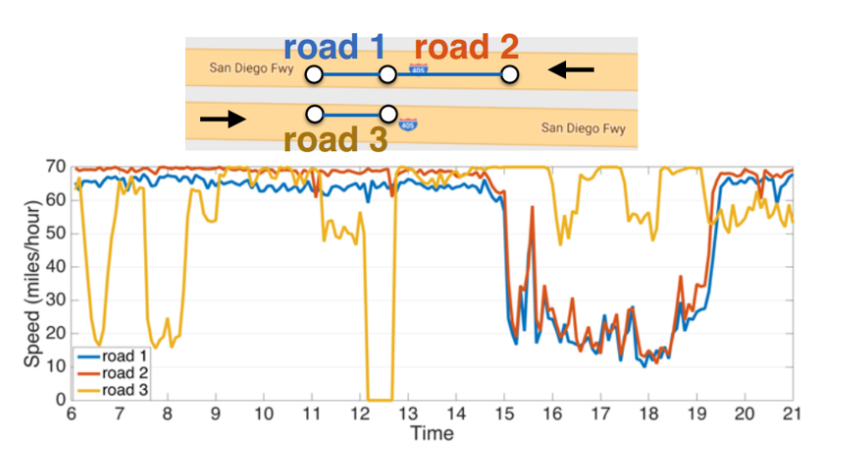
\includegraphics[width=1\textwidth]{../材料/pic/真实车流量.png} %中括号中的参数是设置图片充满文档的大小,你也可以使用小数来缩小图片的尺寸。
            %\caption{推荐系统} %caption是用来给图片加上图题的
            %\label{wolf} %这是添加标签,方便在文章中引用图片。
        \end{figure}%figure环境
    \end{columns}
    
\end{frame}